%\documentclass{clases}
\documentclass[a4paper,12pt, oneside]{book}
\usepackage[skins,minted]{tcolorbox}
\usepackage[utf8]{inputenc}
\usepackage[T1]{fontenc}
\usepackage[spanish, es-tabla]{babel}
\languageshorthands{spanish}
%\usepackage{lmodern} % Usa las fuentes modernas de LaTeX
\usepackage[numbers]{natbib}
%\usepackage{morewrites}
\usepackage{inconsolata}
\usepackage{mdframed}
\usepackage{minted}
\usepackage{bm}
\usepackage{listingsutf8}
\usepackage{subcaption}
\usepackage{amsmath}
\usepackage{amssymb}
\usepackage{graphicx}
\usepackage{hyperref}
\usepackage{longtable}
\usepackage{tabularx}
\usepackage{threeparttable}
\usepackage{array}    % Necesario para centrar horizontal y verticalmente
\usepackage{xcolor}
\usepackage{pdfpages}
%\usepackage{color}
\usepackage{fancyhdr}
\usepackage{menukeys}
\usepackage{appendix}
\usepackage{fontawesome}
\usepackage{comment}
\usepackage{caption}
\usepackage{setspace}
\usepackage[explicit]{titlesec}
\usepackage{booktabs}
\usepackage[a4paper,margin=2cm]{geometry}

%\geometry{top=3cm, bottom=3cm, left=4cm, right=2cm} % Si lo quieres imprimir

\definecolor{green1}{HTML}{1dae28}
\definecolor{green2}{HTML}{afd095}
\definecolor{lightgray}{gray}{0.9}
\definecolor{orange}{RGB}{18,84,183}
\definecolor{titulo}{gray}{0.75}
\definecolor{gray97}{gray}{.97}
\definecolor{gray75}{gray}{.75}
\definecolor{gray45}{gray}{.45}
\definecolor{advertencia}{RGB}{255,178,102}
\definecolor{colorturqueza}{RGB}{178,223,238}
\definecolor{mintedbackground}{rgb}{0.95,0.95,0.95}
\definecolor{lbcolor}{rgb}{0.95,0.95,0.95}
\definecolor{mintedframe}{rgb}{0.0,0.0,0.0}
\definecolor{codebg}{rgb}{0.96,0.96,0.96}
\definecolor{colorurls}{RGB}{107,17,17}
\definecolor{colorsql}{RGB}{255,245,245}
\definecolor{colorreferences}{RGB}{48,134,3}
\definecolor{titulo}{gray}{0.65}			%------ color para fondo del titulo de tablas.

\hypersetup{
	%bookmarks=true,         % show bookmarks bar?
	unicode=true,          % non-Latin characters in Acrobat’s bookmarks
	pdftoolbar=true,        % show Acrobat’s toolbar?
	pdfmenubar=true,        % show Acrobat’s menu?
	pdffitwindow=false,     % window fit to page when opened
	pdfstartview={FitH},    % fits the width of the page to the window
	pdftitle={Reporte final de Robótica},    % title
	%	pdfauthor={},     % author
	pdfsubject={Reporte final de Robótica},   % subject of the document
	%pdfcreator={pdfTeX 3.14159265-2.6-1.40.16 (TeX Live 2016/dev)},   % creator of the document
	%pdfproducer={Panel HJ 2017}, % producer of the document
	pdfkeywords={Manipulador industrial} {Robotica} {ros} {gazebo}, % list of keywords
	%pdfnewwindow=true,      % links in new PDF window
	colorlinks=true,       % false: boxed links; true: colored links
	linkcolor=black,          % color of internal links (change box color with linkbordercolor)
	citecolor=colorreferences,        % color of links to bibliography
	filecolor=magenta,      % color of file links
	urlcolor=blue,           % color of external links
	linkbordercolor={0 0 0}
}

\lstset{
	inputencoding=utf8,
	language=Python,
	frame=Ltb,
	tabsize=2,
	framerule=0pt,
	aboveskip=0.5cm,
	framextopmargin=0pt,
	framexbottommargin=0pt,
	framexleftmargin=0.4cm,
	framesep=0pt,
	rulesep=.0pt,
	backgroundcolor=\color{gray97},
	rulesepcolor=\color{blue},
	%
	stringstyle=\ttfamily,
	showstringspaces = false,
	basicstyle=\small\ttfamily,
	commentstyle=\color{gray45},
	keywordstyle=\bfseries,
	%
	numbers=none,
	numbersep=15pt,
	numberstyle=\tiny,
	numberfirstline = false,
	breaklines=true
}

\setminted[matlab]{%
	breaklines=true,       % activa el ajuste de línea
	breakanywhere=true,    % permite partir en cualquier punto si no hay espacios
	breaksymbolleft=,      % quita el símbolo de continuación
	autogobble            % elimina sangrías comunes
%	fontsize=\footnotesize % reduce tamaño de fuente para que quepa mejor
}

\setminted[bash]{
	bgcolor=mintedbackground,
	fontfamily=tt,
	linenos=true,
	numberblanklines=true,
	numbersep=11pt,
	numbersep=2pt,
	gobble=0,
	frame=leftline,
	framesep=2mm,
	funcnamehighlighting=false,
	tabsize=4,
	obeytabs=false,
	samepage=false,
	showspaces=false,
	showtabs =false,
	texcl=false,
	baselinestretch=1.2,
	fontsize=\footnotesize,
	breaklines=true,
	breaksymbolleft=\ 
}
%\setminted{%
%	breaklines,
%	breaksymbolleft=,      % vacía la marca de continuación
%	breaksymbolright=      % también limpia el símbolo a la derecha
%}


\lstdefinestyle{consola}{
	basicstyle=\footnotesize\bf\ttfamily,
	backgroundcolor=\color{gray75},
}	
\definecolor{gray}{rgb}{0.4,0.4,0.4}
\definecolor{darkblue}{rgb}{0.0,0.0,0.6}
\definecolor{cyan}{rgb}{0.0,0.6,0.6}
\lstset{language=XML}

\lstdefinelanguage{XML}{
	morestring=[b]",
	tabsize=2,
	breaklines=true,
	morestring=[s]{>}{<},
	morecomment=[s]{<?}{?>},
	stringstyle=\color{black},
	identifierstyle=\color{darkblue},
	keywordstyle=\color{cyan},
	numbers=left,
	morekeywords={xmlns,version,type}% list your attributes here
}

\lstdefinestyle{C}{language=C}
\lstdefinestyle{XML}{language=XML}

\DeclareMathOperator{\diag}{diag}

\newtcblisting{terminal}[2][]{
	listing engine=minted,
	listing only,
	#1,
	title=#2,
	minted language=bash,
	colback=mintedbackground,
	top=0mm,
	bottom=0mm
}

\newtcblisting{matlabcode}[2][]{%
  	listing engine=minted,
	listing only,
	title=#2,
	minted language=matlab,
	minted options={%
		linenos,            % activa numeración de líneas
		numbersep=1mm,      % separación texto–números
		breaklines,         % opcional: ajuste automático
		autogobble,          % opcional: recortar sangrías
		frame=leftline,     % línea vertical a la izquierda del bloque
		framesep=1mm,
		tabsize=4,
	},
%	colback=gray!5,
%	colframe=black!70,
	top=0mm,
	bottom=0mm
	#1
}


\newtcblisting{latexcode}[2][]{%
	listing engine=minted,
	listing only,
	title=#2,
	minted language=latex,
	minted options={%
		linenos,            % activa numeración de líneas
		numbersep=1mm,      % separación texto–números
		breaklines,         % opcional: ajuste automático
		autogobble,          % opcional: recortar sangrías
		frame=leftline,     % línea vertical a la izquierda del bloque
		framesep=1mm,
		tabsize=4,
	},
	%	colback=gray!5,
	%	colframe=black!70,
	top=0mm,
	bottom=0mm
	#1
}


\newtcblisting{consolestyle}[2][]{enhanced, listing engine=minted, 
	listing only,#1, title=#2, minted language=bash, 
	coltitle=mintedbackground!35!black, 
	fonttitle=\ttfamily\footnotesize,
	sharp corners, top=0mm, bottom=0mm,
	title code={\path[draw=mintedframe, dashed, fill=mintedbackground](title.south west)--(title.south east);},
	frame code={\path[draw=mintedframe, fill=mintedbackground](frame.south west) rectangle (frame.north east);}
}

\newenvironment{doble}
{\doublespacing
}

%\newcounter{comando}[section]
%\newenvironment{comando}[1][]{\refstepcounter{comando}\par\medskip
	%	\noindent \textbf{Comando~\thecomando. #1} \rmfamily}{\medskip}
%\begin{terminal}{#1}

%\end{terminal}
%}{\medskip}

\graphicspath{{img/}{tablas/}{portada/}}  % Las imágenes se buscarán en la carpeta "img"

\addto\captionsspanish{\renewcommand{\contentsname}{Índice}}

\def\CC{{C\nolinebreak[4]\hspace{-.05em}\raisebox{.4ex}{\tiny\bf ++ \space}}}
\def\Cc{{C\nolinebreak[4]\hspace{-.05em}\raisebox{.4ex}{\tiny\bf ++}}}
\newcommand{\ffolder}[1]{\menu{\faFolderO \space #1}}
\newcommand{\ffile}[1]{\menu{\faFileO \space #1}}
\newcommand{\folder}{\faFolderO \space}
\newcommand{\file}{\faFileO \space}
\newcommand{\world}{\faGlobe \space}
\newcommand{\wworld}[1]{\menu{\faGlobe \space #1}}
\newcommand{\SB}{\{B\}} % Define el sistema del cuerpo
\newcommand{\SI}{\{I\}} % Define el sistema inercial

\newcounter{actividad} % Define un contador llamado "actividad"

\newfloat{Comando}{h}{lot}[chapter]

\renewcommand{\tablename}{Tabla}
\renewcommand{\listtablename}{Índice de tablas}
\renewcommand\listingscaption{Código}
\newcommand{\code}[1]{\colorbox{lightgray}{\texttt{#1}}}

\renewcommand\lstlistingname{Código}
\renewcommand{\appendixname}{Anexo}
\renewcommand{\appendixtocname}{Anexos}
%\renewcommand{\appendixpagename}{Anexo}
\renewcommand\labelitemi{$\bullet$}

\begin{document}
	% Aquí se encuentra el archivo con la portada
	\begin{titlepage}
	\centering
	%-------------------------------------------
	% Logos en una tabla: izquierda, centro y derecha
	\begin{tabular}{@{}p{0.3\textwidth} p{0.3\textwidth} p{0.3\textwidth}@{}}
		
\includegraphics[height=2cm]{tecnm} & 
		\centering 
\includegraphics[height=1.5cm]{SEP} & 
		\raggedleft 
\includegraphics[height=2cm]{ith.jpg} \\
	\end{tabular}
	
	\vspace{2em}
	
	\noindent
	%-------------------------------------------
	%	Información institucional y académica (esquina superior izquierda)
	\begin{minipage}[t]{0.6\textwidth}
		\raggedright
		\small \textbf{%
			Instituto Tecnológico de Hermosillo\\
			Materia: Robótica\\
			Profesor: Medina Gil Lamadrid, Jesús Iván%
		}
	\end{minipage}%
	\hfill
	%	fecha actual (esquina superior derecha), en letras pequeñas y en negrita.
	\begin{minipage}[t]{0.3\textwidth}
		\raggedleft
		\small \textbf{\today}
	\end{minipage}
	
	\vspace{2em}
	
	%-----------------------------------------
	% Unidad y Título de la tarea en letras grandes y en negrita
	{\large \textbf{Unidad 1: Morfología del robot}}\\
	{\Huge \textbf{Cómo hacer un reporte con \LaTeX}}
		
	\vspace{1em}
	
	%---------------------------------------
	% Tabla con la información del equipo
	%---------------------------------------
	% Encabezado del equipo
	\begin{center}
		{\Large \textbf{Equipo N}}
	\end{center}
	
	\vspace{1em}
	
	% Tabla de integrantes:
	% Cada fila contiene: foto (columna izquierda) y datos del integrante (columna derecha)
	\begin{center}
		\begin{tabular}{c c}
			\begin{tabular}{c}
				
\includegraphics[height=3cm]{perfil1.jpg} \\
				\textbf{Apellido1},\\ Nombre1 \\ \texttt{correo1@ejemplo.com} \\ Teléfono: (opcional)
			\end{tabular} &
			\begin{tabular}{c}
				
\includegraphics[height=3cm]{perfil2.jpg} \\
				\textbf{Apellido2,}\\ Nombre2 \\ \texttt{correo2@ejemplo.com} \\ Teléfono: (opcional)
			\end{tabular} \\ \vspace{2em}
			\begin{tabular}{c}
				
\includegraphics[height=3cm]{perfil3.jpg} \\
				\textbf{Apellido3,}\\ Nombre3 \\ \texttt{correo3@ejemplo.com} \\ Teléfono: (opcional)
			\end{tabular} &
			\begin{tabular}{c}
				
\includegraphics[height=3cm]{perfil4.jpg} \\
				\textbf{Apellido4,}\\ Nombre4 \\ \texttt{correo4@ejemplo.com} \\ Teléfono: (opcional)
			\end{tabular}
		\end{tabular}
	\end{center}

\end{titlepage}

	\onehalfspacing
	\frontmatter
	\pagestyle{plain}  % numeración en páginas preliminares
	\titleformat{\chapter}
	{\bfseries\huge}
	{}
	{0pt}
	{~\raisebox{-1.5pt}{}
	\\\filleft #1 \\\vspace{.25cm}\titlerule[1.5pt]}
	
	% ---------------------------------------
	% índices
%	\clearpage   % o \cleardoublepage, según prefieras
	\newpage
	\phantomsection    % crea un nuevo destino para hyperref
	\addcontentsline{toc}{chapter}{Índice general}
	\tableofcontents
	
%	\clearpage
	\newpage
	\phantomsection
	\addcontentsline{toc}{chapter}{Índice de figuras}
	\listoffigures
	
	\hypersetup{
		linkcolor=red
	}
	
	% ---------------------------------------
	% Estilo de encabezado y pie de página
	\mainmatter
	\pagestyle{fancy}
	\fancyhead{}
	\fancyhead[L]{\leftmark}
	\fancyhead[R]{}
	\fancyfoot[L]{\parbox[l]{\textwidth-1cm}{\rightmark}}
	\fancyfoot[C]{}
	\fancyfoot[R]{\thepage}
	\renewcommand{\footrulewidth}{0.5pt}
	%\fancyfoot[RO,LE]{Diseño de modelo para simulación 3D de VANT tipo cuadricóptero}
	
	\titleformat{\chapter}
	{\bfseries\huge}
	{}
	{0pt}
	{\titlerule[3pt]~\raisebox{-1.5pt}{\sc{\chaptername}~\thechapter}~\titlerule[3pt]%
		\\\vspace{.05cm}\titlerule\\\filcenter #1 \\\vspace{.25cm}\titlerule}
	
	% Capítulo 1: Introducción
	\chapter{Desarrollo} \label{chap:desarrollo}
En este capítulo hablarán sobre el proyecto del robot que hicieron y los pasos para llevarlo a cabo, así como algunas funciones de Matlab. Que lo hicieron con Solidworks y lo convirtieron a URDF para usarlo con ROS.
	
	% Capítulo 2: Marco Teórico
	\chapter{Desarrollo} \label{chap:desarrollo}
En este capítulo hablarán sobre el proyecto del robot que hicieron y los pasos para llevarlo a cabo, así como algunas funciones de Matlab. Que lo hicieron con Solidworks y lo convirtieron a URDF para usarlo con ROS.
	
		\section{Cinemática} \label{sec:cinematica}

La cinemática es una rama de la mecánica clásica que se encarga del estudio del movimiento de los cuerpos sin considerar las fuerzas que lo causan. Es decir, se centra en describir cómo se mueven los objetos, especificando variables como posición, velocidad y aceleración, generalmente en función del tiempo.

\cite{conceptoCinematica} dice lo que es la cinemática.

\textbf{Definición de Cinemática (según fuentes académicas y MATLAB).}


Según libros clásicos de robótica y mecánica, como "Introduction to Robotics: Mechanics and Control" de John J. Craig, la cinemática en el contexto de la robótica se refiere al estudio de la posición y orientación de un robot (especialmente de su efector final) respecto a un marco de referencia, y cómo cambian estas variables con respecto al movimiento de sus articulaciones.

En el entorno de MATLAB, particularmente en su toolbox de robótica (Robotics System Toolbox), la cinemática también se entiende como el modelo matemático que relaciona los parámetros articulares de un robot con la posición y orientación de su efector final. MATLAB proporciona funciones como:

getTransform(robot, configuration, endEffector) para obtener la cinemática directa.

Algoritmos de solución de cinemática inversa con objetos como inverseKinematics.

\subsection{Cinemática Directa}
La definición geométrica de la cinemática de robots se basa en representar el movimiento de cada eslabón (o segmento) de un manipulador mediante transformaciones geométricas, típicamente matrices de transformación homogénea. El método más comúnmente usado para modelar estas transformaciones es el algoritmo de Denavit-Hartenberg (D-H).

En \cite{uclmFKIK} se muestran los conceptos de cinemática directa.

\textbf{Parametros DH}
\begin{table}[H]\
	\centering
	\begin{tabular}{|c|c|p{9cm}|}
		\hline
		\textbf{Parámetro} & \textbf{Símbolo} & \textbf{Descripción} \\
		\hline
		Longitud del eslabón & $a_i$ & Distancia entre los ejes $Z_{i-1}$ y $Z_i$, medida a lo largo del eje $X_i$. \\
		\hline
		Ángulo del eslabón & $\alpha_i$ & Ángulo entre los ejes $Z_{i-1}$ y $Z_i$, medido alrededor del eje $X_i$. \\
		\hline
		Desplazamiento del eslabón & $d_i$ & Distancia entre los orígenes de los sistemas de coordenadas $O_{i-1}$ y $O_i$, medida sobre el eje $Z_{i-1}$. \\
		\hline
		Ángulo articular & $\theta_i$ & Ángulo entre los ejes $X_{i-1}$ y $X_i$, medido alrededor del eje $Z_{i-1}$. \\
		\hline
	\end{tabular}
	\caption{Parámetros del modelo Denavit-Hartenberg}
	\label{tabla:dh}
\end{table}


\textbf{Matriz de transformación homogénea (Ai)}


\[
\mathbf{A}_i =
\begin{bmatrix}
	\cos\theta_i & -\sin\theta_i\cos\alpha_i & \sin\theta_i\sin\alpha_i & a_i\cos\theta_i \\
	\sin\theta_i & \cos\theta_i\cos\alpha_i & -\cos\theta_i\sin\alpha_i & a_i\sin\theta_i \\
	0            & \sin\alpha_i              & \cos\alpha_i              & d_i \\
	0            & 0                         & 0                         & 1
\end{bmatrix}
\]



\subsection{Cinemática Diferencial}

La \textbf{cinemática diferencial} estudia cómo las velocidades articulares de un robot afectan la velocidad lineal y angular del efector final. Esta relación se describe mediante una herramienta fundamental llamada la \textbf{matriz Jacobiana}.

Cinemática diferencial \cite{roboticossCinematica}.

Dado un robot con $n$ grados de libertad y un vector de variables articulares $\boldsymbol{q} = [q_1, q_2, \dots, q_n]^T$, y una función $\boldsymbol{x} = f(\boldsymbol{q})$ que representa la posición y orientación del efector final, se define la relación diferencial como:

\[
\dot{\boldsymbol{x}} = \mathbf{J}(\boldsymbol{q}) \, \dot{\boldsymbol{q}}
\]

donde:
\begin{itemize}
	\item $\dot{\boldsymbol{x}}$ es el vector de velocidad del efector final,
	\item $\dot{\boldsymbol{q}}$ es el vector de velocidades articulares,
	\item $\mathbf{J}(\boldsymbol{q})$ es la matriz Jacobiana.
\end{itemize}

\subsection*{Definición del Jacobiano}

La \textbf{matriz Jacobiana} se define como la matriz de derivadas parciales que relaciona cambios infinitesimales en las variables articulares con los cambios en la posición del efector:

\[
\mathbf{J} = \frac{\partial \boldsymbol{x}}{\partial \boldsymbol{q}} =
\begin{bmatrix}
	\frac{\partial x_1}{\partial q_1} & \cdots & \frac{\partial x_1}{\partial q_n} \\
	\vdots & \ddots & \vdots \\
	\frac{\partial x_m}{\partial q_1} & \cdots & \frac{\partial x_m}{\partial q_n}
\end{bmatrix}
\]

Para manipuladores tridimensionales, el Jacobiano se divide comúnmente en dos componentes:

\[
\mathbf{J} =
\begin{bmatrix}
	\mathbf{J}_v \\
	\mathbf{J}_\omega
\end{bmatrix}
\]

donde:
\begin{itemize}
	\item $\mathbf{J}_v$ relaciona las velocidades articulares con la velocidad lineal del efector final.
	\item $\mathbf{J}_\omega$ relaciona las velocidades articulares con la velocidad angular.
\end{itemize}

\subsection*{Importancia del Jacobiano}

El Jacobiano es esencial en robótica porque:
\begin{itemize}
	\item Permite calcular la velocidad cartesiana del efector a partir de velocidades articulares.
	\item Ayuda a identificar y evitar \textbf{singularidades}, donde el robot pierde movilidad instantánea.
	\item Es fundamental en el \textbf{control en espacio operativo}, donde se desea controlar directamente la velocidad del efector.
	\item Se usa en dinámica para relacionar fuerzas y torques mediante la transposición del Jacobiano.
\end{itemize}

\subsection*{Uso en MATLAB}

En MATLAB, utilizando el \textit{Robotics System Toolbox}, se puede calcular el Jacobiano geométrico de un robot con:

\begin{verbatim}
	J = geometricJacobian(robot, config, endEffectorName);
\end{verbatim}

Este comando devuelve la matriz Jacobiana evaluada en la configuración deseada del robot.


\subsection{Cinemática Inversa}


La \textbf{cinemática inversa} consiste en encontrar el conjunto de variables articulares $\boldsymbol{q}$ que permiten alcanzar una posición y orientación deseadas del efector final $\boldsymbol{x}_d$. Matemáticamente, se plantea como:

\[
\text{Dado: } \boldsymbol{x}_d = f(\boldsymbol{q}) \quad \Rightarrow \quad \text{Hallar: } \boldsymbol{q}
\]

A diferencia de la cinemática directa, este problema puede tener múltiples soluciones, una sola o ninguna, dependiendo de la geometría del manipulador y de su configuración actual.

\subsection*{Método basado en el Jacobiano y el Gradiente}

Una forma común de resolver la cinemática inversa de manera iterativa es minimizar el error:

\[
\boldsymbol{e}(\boldsymbol{q}) = \boldsymbol{x}_d - f(\boldsymbol{q})
\]

El gradiente del error cuadrático respecto a las variables articulares está relacionado con el Jacobiano:

\[
\frac{\partial}{\partial \boldsymbol{q}} \left\| \boldsymbol{e}(\boldsymbol{q}) \right\|^2 = -2 \mathbf{J}^T(\boldsymbol{q}) \boldsymbol{e}(\boldsymbol{q})
\]

Esto lleva al \textbf{método del Jacobiano transpuesto}:

\[
\boldsymbol{q}_{k+1} = \boldsymbol{q}_k + \alpha \mathbf{J}^T(\boldsymbol{q}_k) \boldsymbol{e}(\boldsymbol{q}_k)
\]

donde $\alpha$ es un escalar que controla el paso de la iteración.



		
		\section{ROS} \label{sec:ros}
ROS provee los servicios estándar de un sistema operativo tales como abstracción del hardware, control de dispositivos de bajo nivel, implementación de funcionalidad de uso común, paso de mensajes entre procesos y mantenimiento de paquetes.
\begin{figure}[h]
	\centering
	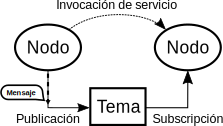
\includegraphics[width=0.5\linewidth]{img/ROS_concepts}
	\caption{Diagrama de comunicación de ROS}
	\label{fig:rosconcepts}
\end{figure}

 \href{https://ubuntu.com/robotics/what-is-ros}{página de Ubuntu} \cite{https://wiki.ros.org/ROS/Tutorials/UnderstandingTopics}.


\subsection{Nodo (Node)}

En ROS (Robot Operating System), un \textbf{nodo} es una unidad de procesamiento que ejecuta una función específica del sistema robótico. Los nodos pueden publicar información, suscribirse a otros nodos, o bien intercambiar información a través de servicios.


\subsection{Tema (Topic)}

Un \textbf{tema} es un canal de comunicación utilizado para el envío de datos entre nodos de forma asincrónica. Un nodo puede publicar mensajes en un tema, mientras que otros nodos pueden suscribirse a ese tema para recibir los datos. Esta es la forma más común de comunicación en ROS.
 
 
\begin{itemize}
	\item \textbf{Publicador:} nodo que envía datos a un tema.
	\item \textbf{Suscriptor:} nodo que recibe datos de un tema.
\end{itemize}


\subsection{Mensaje (Message)}

Los \textbf{mensajes} son estructuras de datos estandarizadas que se transmiten a través de los temas. Pueden incluir tipos de datos como enteros, flotantes, vectores, matrices, imágenes, etc. Los tipos de mensajes están predefinidos en ROS y se agrupan por paquetes, como \texttt{std\_msgs}, \texttt{sensor\_msgs}, \texttt{geometry\_msgs}, entre otros.


\subsection{Servicio (Service)}

Un \textbf{servicio} en ROS es una forma de comunicación sincrónica que sigue el modelo de cliente-servidor. Un nodo ofrece un servicio y otro nodo lo invoca. La comunicación ocurre mediante una solicitud y una respuesta. Los servicios se usan cuando se necesita una operación puntual y no continua.


\begin{itemize}
	\item \textbf{Cliente:} nodo que solicita el servicio.
	\item \textbf{Servidor:} nodo que responde a la solicitud.
\end{itemize}


\subsection{Gazebo}


\textbf{Gazebo} es un simulador 3D que permite probar robots en entornos virtuales realistas. Se integra con ROS para simular sensores, actuadores, objetos y dinámicas físicas. Gazebo actúa como un nodo que publica datos (como imágenes de cámaras, posiciones, fuerzas) en temas de ROS, permitiendo desarrollar algoritmos sin usar hardware real.


\subsection{RViz}

\textbf{RViz} (ROS Visualization) es una herramienta de visualización para ROS que permite observar el estado del robot, sus sensores y el entorno en un espacio tridimensional. Se suscribe a diversos temas del sistema y muestra información como:


\begin{itemize}
	\item Modelos del robot.
	\item Datos de sensores (cámaras, LIDAR).
	\item Trayectorias y mapas.
	\item Marcos de referencia (TF).
\end{itemize}


\subsection*{Resumen}
\begin{table}[H]
	\centering
	\begin{tabular}{|l|p{10cm}|}
		\hline
		\textbf{Elemento} & \textbf{Descripción} \\
		\hline
		Nodo & Proceso que realiza una tarea específica (ej. lectura de sensor, control de motor). \\
		Tema & Canal de comunicación asincrónico entre nodos. \\
		Mensaje & Estructura de datos que se transmite mediante un tema. \\
		Servicio & Comunicación sincrónica mediante solicitud y respuesta. \\
		Gazebo & Simulador físico 3D que emite datos hacia ROS. \\
		RViz & Visualizador 3D de datos del robot en tiempo real. \\
		\hline
	\end{tabular}
	\caption{Resumen de elementos clave en la comunicación de ROS}
\end{table}

		
		\section{Dinámica} \label{sec:dinamica}

La verdad, no les expliqué mucho sobre esta unidad, pero pueden hablar sobre las ecuaciones que vienen en el powerpoint (el cual subí tarde porque se me corrompió)

Hablen sobre el modelo dinámico estandar de un robot, la matriz de masa o inercia, la matriz de coriolis y el vector de gravedad. 

\subsection{Matriz de masa o inercia}
Expliquen cómo el vector de masa o inercia define la aceleración máxima.

\subsection{Matriz de coriolis}

\subsection{Vector de gravedad}

Expliquen por qué el vector de gravedad en su valor máximo (cuando el robot está extendido horizontalmente) debe ser contrarrestado con la fuerza de cada motor

\subsection{Fricción}
Expliquen qué es la fricción en general.

\subsubsection{Fricción estática o seca}

\subsubsection{Fricción dinámica o viscosa}

\subsection{Perturbaciones}
Aquí expliquen qué es una perturbación en general sin profundizar mucho.
		
		%\section{Control} \label{sec:control}
%Algún día lograré explicar bien el Control de su robot, pero este semestre no será supongo. Así que pueden comentar el input de esta parte, pero igual pueden intentar explicar esto.
%

	
	% Capítulo 3: Desarrollo
	\chapter{Desarrollo} \label{chap:desarrollo}
En este capítulo hablarán sobre el proyecto del robot que hicieron y los pasos para llevarlo a cabo, así como algunas funciones de Matlab. Que lo hicieron con Solidworks y lo convirtieron a URDF para usarlo con ROS.
	
		\section{Características del Robot} \label{sec:caracteristicas_del_robot}


En esta sección se describe la estructura cinemática del robot utilizando el método de Denavit-Hartenberg (DH). Este método permite representar la geometría del manipulador mediante cuatro parámetros para cada articulación o eslabón, facilitando la formulación de la cinemática directa e inversa.

\subsection*{Descripción de los parámetros}

Los parámetros utilizados son los siguientes:

\begin{itemize}
	\item \textbf{\(\theta\)}: Ángulo de rotación alrededor del eje \(z\) (solo para articulaciones rotacionales).
	\item \textbf{\(d\)}: Desplazamiento a lo largo del eje \(z\) (solo para articulaciones prismáticas).
	\item \textbf{\(a\)}: Longitud del eslabón o distancia entre los ejes \(z\), medida sobre el eje \(x\).
	\item \textbf{\(\alpha\)}: Ángulo de torsión entre ejes \(z\), medido sobre el eje \(x\).
	\item \textbf{Tipo}: Tipo de articulación. 'r' indica rotacional y 'p' prismática.
	\item \textbf{\(q_{\text{min}}\) y \(q_{\text{max}}\)}: Límites inferiores y superiores del rango de movimiento de cada articulación.
	\item \textbf{\(\dot{q}_{\text{max}}\)}: Velocidad máxima permitida para la articulación.
	\item \textbf{\(\ddot{q}_{\text{max}}\)}: Aceleración máxima permitida.
	\item \textbf{\(\tau\)}: Torque máximo para articulaciones rotacionales o fuerza máxima para articulaciones prismáticas.
	\item \textbf{\(\mu_s\)}: Coeficiente de fricción estática.
	\item \textbf{\(\mu_k\)}: Coeficiente de fricción dinámica.
\end{itemize}

\subsection*{Tabla de parámetros DH y límites dinámicos}

	
	\section*{Parámetros Denavit-Hartenberg del Robot \texttt{robot0}}
	
	La siguiente tabla representa los parámetros Denavit-Hartenberg modificados del robot denominado \texttt{robot0}, el cual tiene 6 articulaciones rotacionales.
	
	\begin{table}[h!]
		\centering
		\begin{tabular}{ccccccccccc}
			\toprule
			\textbf{$\theta$} & \textbf{$d$} & \textbf{$a$} & \textbf{$\alpha$} & \textbf{tipo} & \textbf{min (°)} & \textbf{max (°)} & \textbf{$\dot{q}_{\text{max}}$ (°/s)} & \textbf{$\ddot{q}_{\text{max}}$ (°/s²)} \\
			\midrule
			2   & 39.91 & 0     & -90 & r & -90 & 90 & 180 & 360 \\
			-90 & 0     & 44.8  & 0   & r & -90 & 90 & 180 & 360 \\
			0   & 0     & 4.197 & -90 & r & -90 & 90 & 180 & 360 \\
			0   & 45.1  & 0     & 90  & r & -90 & 90 & 180 & 360 \\
			90  & 0     & 9.5   & 0   & r & -90 & 90 & 180 & 360 \\
			\bottomrule
		\end{tabular}
		\caption{Parámetros DH del robot \texttt{robot0}. Todos los ángulos están en grados y las longitudes en centimetros.}
	\end{table}
	
	\textbf{Descripción de cada parámetro:}
	\begin{itemize}
		\item $\theta$: Ángulo de rotación en torno al eje z del eslabón anterior.
		\item $d$: Desplazamiento a lo largo del eje z del eslabón anterior.
		\item $a$: Longitud del eslabón, medida en la dirección del eje x.
		\item $\alpha$: Ángulo entre los ejes z consecutivos, medido alrededor del eje x.
		\item \textbf{tipo}: Indica si la articulación es rotacional (\texttt{r}).
		\item \textbf{min} y \textbf{max}: Límites del ángulo de cada articulación en grados.
		\item $\dot{q}_{\text{max}}$: Velocidad angular máxima permitida por articulación (°/s).
		\item $\ddot{q}_{\text{max}}$: Aceleración angular máxima permitida por articulación (°/s²).
	\end{itemize}
	
	\textbf{Interpretación:}  
	Este conjunto de parámetros define completamente la estructura geométrica y las limitaciones cinemáticas del robot. La uniformidad de los valores de velocidad y aceleración máxima indica que el robot fue modelado con restricciones homogéneas en cada articulación, lo cual es útil para simulaciones o análisis de control.
	



		
			\subsection{Partes} \label{subsec:partes}
Información de las piezas del robot. 

\textbf{1-Parametros del motor NEMA 17}
\begin{figure} [h]
	\centering
	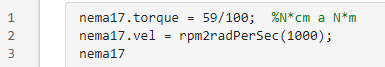
\includegraphics[width=0.7\linewidth]{img/calculomotores1}
	\caption{Parametros del motor NEMA 17}
	\label{fig:calculomotores1}
\end{figure}


-59/100 convierte el torque de 59 N·cm a 0.59 N·m.

-Se usa rpm2radPerSec() para convertir 1000 rpm a radianes por segundo.

-Se imprime el resultado.


\textbf{2-Parametros del motor NEMA 23}
\begin{figure} [h]
	\centering
	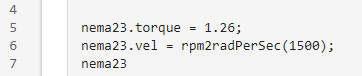
\includegraphics[width=0.7\linewidth]{img/calculomotores2}
	\caption{Parametros del motor NEMA 23}
	\label{fig:calculomotores2}
\end{figure}


-Se inicializa el motor NEMA 23 con su torque y velocidad, ya en unidades estándar del SI.

\newpage
\textbf{3-Parametros del servo}
\begin{figure} [h]
	\centering
	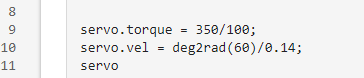
\includegraphics[width=0.7\linewidth]{img/calculomotores3}
	\caption{Parametros del servo}
	\label{fig:calculomotores3}
\end{figure}

-Calcula cuántos rad/s representa girar 60° en 0.14 s.


\textbf{4-Articulación 1: motor NEMA 17 con polea}

\begin{figure} [h]
	\centering
	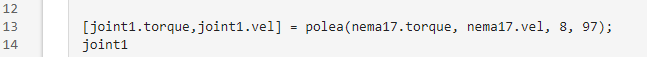
\includegraphics[width=0.7\linewidth]{img/calculomotores4}
	\caption{motor NEMA 17 con polea}
	\label{fig:calculomotores4}
\end{figure}

-Se usa una transmisión por poleas con una entrada de 8 mm y salida de 97 mm.

-Aumenta el torque y reduce la velocidad proporcionalmente.


\textbf{5-Articulación 2: NEMA 23 + polea + engranaje}


\begin{figure} [h]
	\centering
	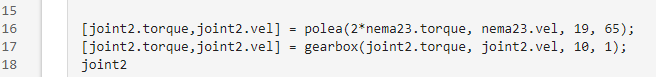
\includegraphics[width=0.7\linewidth]{img/calculomotores5}
	\caption{NEMA 23 + polea + engranaje}
	\label{fig:calculomotores5}
\end{figure}


-Se suman los torques de dos motores NEMA 23.

-Pasa por una polea (19 mm entrada, 65 mm salida) y una caja reductora (relación 10:1).

-El torque aumenta en ambas etapas, la velocidad disminuye.

\newpage
\textbf{6-Articulación 3: NEMA 17 + polea + engranaje}

\begin{figure} [h]
	\centering
	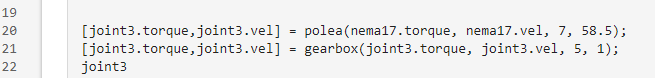
\includegraphics[width=0.7\linewidth]{img/calculomotores6}
	\caption{NEMA 17 + polea + engranaje}
	\label{fig:calculomotores6}
\end{figure}


-Primero, el torque y la velocidad del motor NEMA 17 pasan por una polea con un diámetro de entrada de 7 mm y salida de 58.5 mm.

-Esto incrementa el torque y reduce la velocidad angular en proporción al cociente 58.5/7

-Después, los valores resultantes pasan por una caja reductora con una relación de 5:1.

-Nuevamente, el torque se multiplica por 5, y la velocidad se divide por 5.

-Resultado: aumento significativo del torque y gran reducción de velocidad, ideal para tareas de fuerza con baja velocidad.


\textbf{7-Articulación 4: Motor NEMA 17 con una sola polea}

\begin{figure} [h]
	\centering
	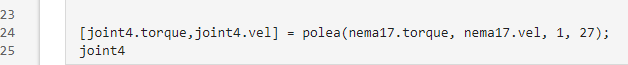
\includegraphics[width=0.7\linewidth]{img/calculomotores7}
	\caption{Motor NEMA 17 con una sola polea}
	\label{fig:calculomotores7}
\end{figure}


-Este caso modela una polea simple con una gran relación 27/1, es decir:

Aumenta 27 veces el torque.

Disminuye la velocidad 27 veces.

-Útil para articulaciones que requieren alta fuerza con muy poca velocidad, como agarres o soportes


\textbf{8-Articulación 5: Servo directamente}


\begin{figure} [h]
	\centering
	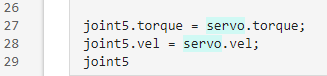
\includegraphics[width=0.7\linewidth]{img/calculomotores8}
	\caption{Servo directamente}
	\label{fig:calculomotores8}
\end{figure}


-No se aplica ni polea ni engranaje.

-Se asignan directamente el torque y la velocidad angular del servo motor a la articulación 5.

-Esto representa un accionamiento directo, normalmente en aplicaciones donde ya se ha diseñado el servo para cumplir con los requerimientos mecánicos de torque y velocidad.


%\subsubsection{Motores} \label{subsubsec:motores}
%Explicarán cuál es el motor que usaron, harán referencia a la hoja de datos, así como las transmisiones (por ejemplo, las de las pinzas) o reductores de velocidad a los que están acoplados. Deben de poner también información como: masa, fuerza o torque máximo, razón de reducción (por ejemplo, 10/1) y la velocidad máxima.
%%\subsubsection{Eslabones} \label{subsubsec:eslabones}
%Pondrán la masa, inercia, longitud y material de cada eslabón.
			
			\subsection{Límites y propiedades dinámicas de las articulaciones} \label{subsec:limites_propiedades}

Básicamente, explicarán lo que aparece en la \autoref{tab:parametros_robot}: Parámetros de Denavit Hartenberg y límites del robot, específicamente lo que aparece después de \code{tipo}. Como no completamos la tarea de dinámica,. pueden comentar esta subsección del documento principal.
		
		\section{Proceso de Cinemática} \label{sec:proceso_cinematica}


La cinemática de un manipulador robótico comprende el estudio del movimiento de sus eslabones sin considerar las fuerzas involucradas. En este trabajo, se abordan los tres tipos principales de análisis cinemático: directo, diferencial e inverso, utilizando un modelo basado en la convención de Denavit-Hartenberg (DH).

\textbf{Cinemática Directa:} Se establecen la orientación y posición inicial del efector final a través de una matriz de transformación homogénea construida a partir de ángulos de Euler. Utilizando los parámetros DH del archivo \texttt{robot2.csv}, se crea una estructura cinemática del robot que permite calcular la pose del efector final dado un conjunto de posiciones articulares. Además, se generan trayectorias cíclicas articulares (posición, velocidad y aceleración) con un periodo definido, que sirven como base para el análisis cinemático y dinámico.

\textbf{Cinemática Diferencial:} A partir de las trayectorias articulares calculadas, se obtiene la evolución temporal de la posición y orientación del efector final. Se implementa el cálculo del Jacobiano geométrico del robot para obtener la velocidad lineal y angular del efector. Asimismo, se calcula la aceleración utilizando la derivada temporal del Jacobiano, aplicando diferencias finitas. Este análisis permite conocer el comportamiento cinemático instantáneo del robot en cada instante de la trayectoria.

\textbf{Cinemática Inversa:} Se plantea el problema de encontrar las configuraciones articulares necesarias para que el efector final siga una trayectoria deseada en el espacio cartesiano. Se resuelve utilizando un algoritmo iterativo basado en el Jacobiano, el cual converge con alta precisión tras varias iteraciones. Se registran los errores finales y la cantidad de iteraciones requeridas, demostrando la efectividad del método.

En conjunto, estos análisis permiten simular, controlar y validar el comportamiento cinemático completo del manipulador robótico, desde las entradas articulares hasta la ejecución precisa de trayectorias en el espacio.

\newpage
\subsection{Cinemática Directa}

\begin{figure} [h]
	\centering
	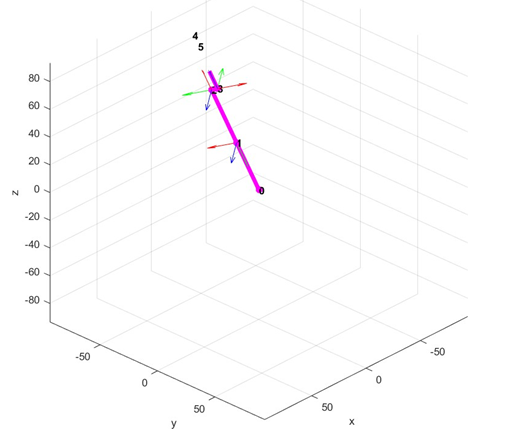
\includegraphics[width=0.7\linewidth]{img/robotcindir}
	\caption{Robot Cinematica Directa}
	\label{fig:robotcindir}
\end{figure}

En esta sección se describe el procedimiento para definir la orientación inicial del efector final del robot, construir la matriz de transformación homogénea de referencia y calcular las trayectorias articulares de forma cíclica.

\subsection*{3.2.1.1. Definición de orientación inicial}

Se definen los ángulos de orientación del efector final respecto a los tres ejes cartesianos:

\begin{verbatim}
	phi = 10;    % Rotación sobre el eje X
	theta = 20;  % Rotación sobre el eje Y
	psi = 30;    % Rotación sobre el eje Z
\end{verbatim}

Estos ángulos, dados en grados, se convierten a radianes y se almacenan como un vector columna:

\begin{verbatim}
	orientacion_inicial = deg2rad([phi; theta; psi]);
	secuencia = "XYZ";
\end{verbatim}

La variable \texttt{secuencia} define el orden de aplicación de las rotaciones según el sistema de ángulos de Euler. En este caso, la secuencia "XYZ" indica que las rotaciones se aplican primero sobre \(X\), luego \(Y\) y finalmente sobre \(Z\).

\subsection*{3.2.1.2. Construcción de la matriz de transformación homogénea inicial}

Se calcula la matriz de rotación utilizando la función \texttt{euler2rotMat} a partir de los ángulos definidos:

\begin{verbatim}
	R = euler2rotMat(orientacion_inicial, secuencia);
\end{verbatim}

Luego, se construye la matriz de transformación homogénea \( A_0 \), que representa la orientación y posición inicial del efector final en el espacio:

\begin{verbatim}
	A0 = [R          posicion_inicial
	zeros(1,3) 1];
\end{verbatim}

\begin{itemize}
	\item \texttt{R}: matriz de rotación \(3 \times 3\)
	\item \texttt{posicion\_inicial}: vector columna \(3 \times 1\) con la posición inicial
	\item \texttt{A0}: matriz homogénea \(4 \times 4\) que define la pose inicial del robot
\end{itemize}

\subsection*{3.2.1.3. Definición del intervalo de tiempo}

Se define un intervalo temporal de 8 segundos con un paso de muestreo de 0.05 s, útil para simular trayectorias continuas:

\begin{verbatim}
	t_inicial = 0;
	t_final = 8;
	t_paso = 0.05;
	t = t_inicial:t_paso:t_final;
\end{verbatim}

\subsection*{3.2.1.4. Lectura de parámetros DH y creación de la estructura del robot}

La estructura cinemática del robot se genera a partir de los parámetros DH almacenados en un archivo CSV:

\begin{verbatim}
	dh = readtable('datos\tabla_DH\robot2.csv');
	robot = crear_robot(dh, A0);
\end{verbatim}

\subsection*{3.2.1.5. Generación de trayectorias articulares}

Finalmente, se genera una trayectoria periódica para los valores articulares \( q \), sus derivadas \( \dot{q} \) (velocidades) y \( \ddot{q} \) (aceleraciones), usando una función cíclica con un periodo de 2 segundos:

\begin{verbatim}
	periodo = 2;    % Periodo del movimiento cíclico
	[q,dq,ddq] = trayectoria_q(robot, t, periodo);
\end{verbatim}

Estas trayectorias se emplean posteriormente para simular el comportamiento dinámico del robot y calcular su cinemática diferencial.


\subsection{Cinemática Diferencial}
Para analizar la cinemática directa del robot, se parte de una tabla de parámetros de Denavit-Hartenberg (DH), la cual contiene la descripción geométrica del manipulador. El archivo \texttt{robot2.csv} contiene los parámetros necesarios para definir cada eslabón del robot: $\theta$, $d$, $a$, y $\alpha$. Estos parámetros son leídos mediante la función \texttt{readtable} y se utiliza una función personalizada \texttt{crear\_robot} que construye el modelo cinemático completo del robot a partir de dicha tabla y una matriz de transformación base $A_0$:

\begin{lstlisting}[language=Matlab]
	dh = readtable('datos\tabla_DH\robot2.csv');
	robot = crear_robot(dh, A0);
\end{lstlisting}

\subsection*{3.2.2.1. Generación de Trayectorias en el Espacio Articular}
Una vez construido el modelo del robot, se generan trayectorias articulares usando perfiles de movimiento cíclico (por ejemplo, funciones senoidales o trapezoidales). El parámetro \texttt{periodo} determina el ciclo del movimiento, y las funciones \texttt{trayectoria\_q} devuelven:

\begin{itemize}
	\item $q(t)$: posición de las articulaciones en función del tiempo,
	\item $\dot{q}(t)$: velocidad articular,
	\item $\ddot{q}(t)$: aceleración articular.
\end{itemize}

Esta información es fundamental para el análisis dinámico del robot, así como para su control. El vector $q(t)$ se puede utilizar como entrada para obtener la pose del efector final mediante la cinemática directa.

\newpage

\subsection{Cinemática Inversa}
\begin{figure} [h]
	\centering
	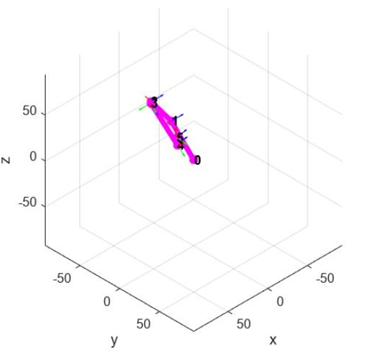
\includegraphics[width=0.7\linewidth]{img/robotcininv}
	\caption{Robot Cinematica Inversa}
	\label{fig:robotcininv}
\end{figure}

\begin{figure} [h]
	\centering
	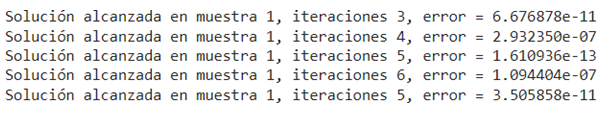
\includegraphics[width=0.7\linewidth]{img/solucionescininv}
	\caption{Soluciones cinematica inversa}
	\label{fig:solucionescininv}
\end{figure}
		
	\textbf{Interpretación:}
	\begin{itemize}
		\item Todos los casos corresponden a la \textbf{muestra 1}, lo que sugiere que se trata de múltiples ejecuciones del algoritmo sobre la misma configuración inicial.
		\item El número de iteraciones varía entre 3 y 6, indicando convergencia rápida en general.
		\item Los errores finales alcanzan valores muy pequeños (del orden de $10^{-11}$ a $10^{-13}$ en algunos casos), lo cual evidencia una alta precisión en la solución encontrada.
		\item Algunos casos presentan errores mayores ($\sim10^{-7}$), lo que puede deberse a condiciones iniciales diferentes, tolerancias del algoritmo o características propias del modelo.
	\end{itemize}
	
	\vspace{0.5cm}
	
	\textbf{Conclusión:}  
	El algoritmo de cinemática inversa utilizado logra encontrar soluciones con alta precisión en un número reducido de iteraciones. Esto sugiere una implementación eficiente y estable, adecuada para aplicaciones de control en tiempo real de robots articulados.
	

		
		%\section{Control} \label{sec:control}
%Algún día lograré explicar bien el Control de su robot, pero este semestre no será supongo. Así que pueden comentar el input de esta parte, pero igual pueden intentar explicar esto.
%

		
		\input{capitulos/Desarrollo/Simulación}
	
	% Capítulo 4: Resultados
	\chapter{Resultados} \label{chap:resultados}
\textbf{Cinematica Directa}
\begin{figure} [h]
	\centering
	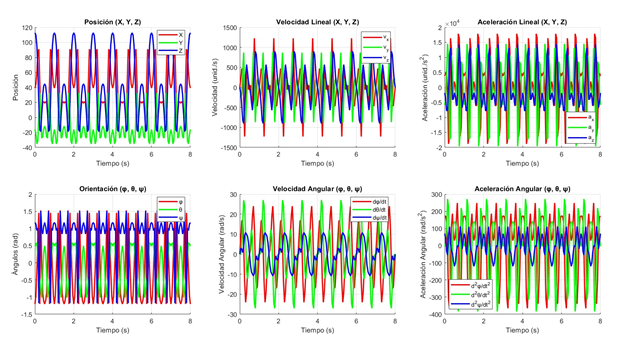
\includegraphics[width=0.7\linewidth]{img/cinematicadirecta}
	\caption{Cinematica directa}
	\label{fig:cinematicadirecta}
\end{figure}

\section*{Análisis de Resultados de Cinemática Directa}


\subsection*{1. Posición Lineal (X, Y, Z)}
La gráfica superior izquierda muestra el movimiento del efector final en los tres ejes cartesianos:


\begin{itemize}
	\item Se observa un movimiento cíclico y oscilatorio, lo que indica una trayectoria periódica en el espacio.
	\item El eje $Z$ (línea azul) tiene mayor amplitud, indicando un movimiento vertical más pronunciado.
\end{itemize}


\subsection*{2. Velocidad Lineal ($\dot{X}$, $\dot{Y}$, $\dot{Z}$)} La gráfica superior central presenta la velocidad en cada dirección:

\begin{itemize}
	\item Las señales son periódicas y muestran una alternancia entre valores positivos y negativos, coherente con el movimiento oscilatorio.
	\item La velocidad alcanza picos de aproximadamente ±1500 unidades/s, lo que indica variaciones rápidas en la trayectoria.
\end{itemize}


\subsection*{3. Aceleración Lineal ($\ddot{X}$, $\ddot{Y}$, $\ddot{Z}$)} La gráfica superior derecha representa la aceleración lineal:

\begin{itemize}
	\item Se observan valores muy altos (hasta ±2e4 unidades/s$^2$), lo que sugiere movimientos rápidos y posibles exigencias dinámicas considerables.
	\item Las aceleraciones son también periódicas y coinciden en fase con las velocidades.
\end{itemize}


\subsection*{4. Orientación (Ángulos de Euler $\phi$, $\theta$, $\psi$)} La gráfica inferior izquierda muestra la orientación del efector final:

\begin{itemize}
	\item Los ángulos de rotación (roll, pitch, yaw) también siguen trayectorias oscilantes.
	\item El ángulo $\phi$ (rojo) presenta las variaciones más marcadas.
\end{itemize}


\subsection*{5. Velocidad Angular}
La gráfica inferior central presenta las velocidades angulares derivadas de la orientación:


\begin{itemize}
	\item Se aprecian oscilaciones periódicas de baja frecuencia con amplitudes consistentes.
	\item Las señales presentan continuidad, lo cual es deseable para evitar movimientos abruptos.
\end{itemize}


\subsection*{6. Aceleración Angular}
Finalmente, la gráfica inferior derecha muestra las aceleraciones angulares:

\begin{itemize}
	\item Se mantiene el comportamiento periódico, pero con valores más elevados y picos que podrían afectar la estabilidad si no se amortiguan.
	\item Refleja las variaciones rápidas en la orientación del efector final.
\end{itemize}


\subsection*{Conclusión}
Este análisis permite verificar que el modelo de cinemática directa está proporcionando una trayectoria suave, periódica y coherente con el comportamiento esperado del robot. Las oscilaciones en posición, velocidad y aceleración indican que se está siguiendo un patrón cíclico, ideal para tareas repetitivas. No obstante, los picos de aceleración lineal y angular sugieren que se deben considerar estrategias de suavizado o limitación de esfuerzos en el diseño del control.

\textbf{Cinematica inversa}


\begin{figure} [h]
	\centering
	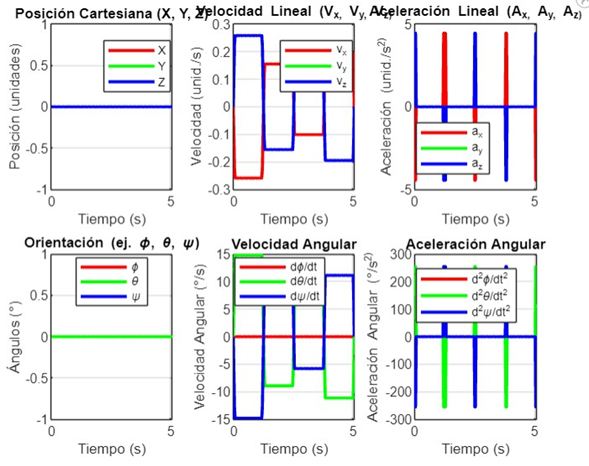
\includegraphics[width=0.7\linewidth]{img/cinematicainvgraficas}
	\caption{Cinematica inversa: Graficas}
	\label{fig:cinematicainvgraficas}
\end{figure}

\begin{figure} [h]
	\centering
	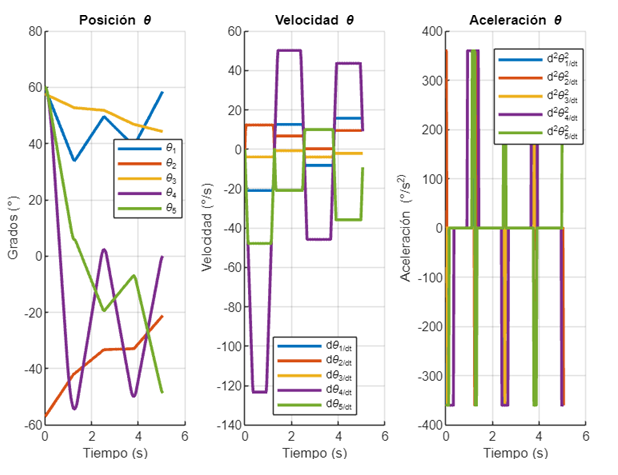
\includegraphics[width=0.7\linewidth]{img/cinematicainvarticular}
	\caption{Cinematica inversa: Articular}
	\label{fig:cinematicainvarticular}
\end{figure}

\newpage
\section*{Análisis de Resultados de Cinemática Inversa}


\subsection*{1. Posición angular $\theta$}
Esta gráfica muestra la posición angular (en grados) de cada articulación en función del tiempo. Cada curva representa el comportamiento de una articulación:


\begin{itemize}
	\item Se observa que las trayectorias son distintas para cada articulación, lo cual indica que cada una realiza un movimiento específico para contribuir al seguimiento de la trayectoria deseada del efector final.
	\item Por ejemplo, $\theta_4$ (línea morada) presenta cambios abruptos y amplios, sugiriendo que dicha articulación realiza movimientos significativos.
\end{itemize}


\subsection*{2. Velocidad angular $\frac{d\theta}{dt}$}

Esta gráfica representa la velocidad angular de las articulaciones (en grados por segundo):


\begin{itemize}
	\item Se observan escalones en las velocidades, indicando que fueron obtenidas mediante diferencias finitas sobre datos muestreados.
	\item Cambios bruscos de velocidad, especialmente en $\theta_4$ y $\theta_5$, pueden generar problemas de control o desgaste mecánico si no se suavizan.
\end{itemize}


\subsection*{3. Aceleración angular $\frac{d^2\theta}{dt^2}$}
La tercera gráfica muestra la aceleración angular (en grados por segundo cuadrado):


\begin{itemize}
	\item Se aprecian valores muy altos (por ejemplo, $\pm 360~^\circ/s^2$), lo que indica transiciones rápidas en la velocidad angular.
	\item Estas aceleraciones escalonadas también sugieren una obtención por diferencias finitas.
	\item Tales picos podrían ser perjudiciales para la operación del robot si no se implementa una trayectoria más suave.
\end{itemize}


\subsection*{Conclusión}
Las gráficas reflejan el comportamiento articular necesario para seguir una trayectoria en el espacio cartesiano. Sin embargo, los cambios abruptos en velocidad y aceleración
indican la necesidad de aplicar técnicas de suavizado como interpolación polinómica (por ejemplo, polinomios cúbicos o quínticos) para garantizar un movimiento más eficiente, seguro y adecuado para el control del robot.


\section*{Análisis de Resultados de Cinemática Inversa Articular}
	
	\section*{Gráfica 1: Posición angular ($\theta$)}
	
	\begin{itemize}
		\item \textbf{Eje X (Tiempo en segundos)}: Representa la evolución temporal (0 a 6 segundos).
		\item \textbf{Eje Y (Grados °)}: Muestra la posición angular de cada articulación en grados.
		\item \textbf{Curvas ($\theta_1$ a $\theta_5$)}: Indican cómo cambian los ángulos articulares en el tiempo.
	\end{itemize}
	
	\textbf{Interpretación:}
	\begin{itemize}
		\item Se observan trayectorias distintas para cada articulación, lo que implica que el movimiento fue calculado individualmente para lograr un posicionamiento específico del efector final (probablemente un robot).
		\item Algunas curvas son suaves, otras muestran cambios abruptos, lo cual puede indicar trayectorias con quiebres o cambios de dirección.
	\end{itemize}
	
	
	\section*{Gráfica 2: Velocidad angular ($d\theta/dt$)}
	
	\begin{itemize}
		\item \textbf{Eje X}: Tiempo (s)
		\item \textbf{Eje Y}: Velocidad angular (°/s)
		\item \textbf{Curvas}: Derivadas de las posiciones angulares (velocidades instantáneas).
	\end{itemize}
	
	\textbf{Interpretación:}
	\begin{itemize}
		\item Se observan velocidades constantes por tramos (formas tipo escalón), lo que indica movimiento a velocidad constante en ciertos intervalos, típico en trayectorias por segmentos lineales.
		\item Cambios abruptos implican transiciones entre movimientos.
	\end{itemize}
	
	
	\section*{Gráfica 3: Aceleración angular ($d^2\theta/dt^2$)}
	
	\begin{itemize}
		\item \textbf{Eje X}: Tiempo (s)
		\item \textbf{Eje Y}: Aceleración angular (°/s²)
		\item \textbf{Curvas}: Segunda derivada de la posición, muestran cómo cambia la velocidad en el tiempo.
	\end{itemize}
	
	\textbf{Interpretación:}
	\begin{itemize}
		\item Aceleraciones son valores muy altos positivos y negativos en intervalos muy breves, lo que sugiere cambios instantáneos de velocidad (lo cual no es físicamente ideal).
		\item Estos picos pueden indicar falta de suavizado en la planificación del movimiento.
	\end{itemize}
	
	
	\section*{Conclusión}
	
	Este conjunto de gráficas parece derivarse de una planificación de trayectorias por puntos (p. ej., control punto a punto en un robot articulado), donde se definieron posiciones deseadas de las articulaciones y se calcularon las velocidades y aceleraciones mediante diferencias finitas.
	
	\textbf{Posibles aplicaciones:}
	\begin{itemize}
		\item Control de robots manipuladores (como brazos robóticos).
		\item Simulación de trayectorias para verificación antes de ejecución física.
		\item Evaluación de la suavidad del movimiento.
	\end{itemize}
	


	
	% Capítulo 5: Conclusiones
	\chapter{Conclusiones} \label{sec:conclusiones}
	\section{Juancito}
Conclusiones y comentarios de Juancito, explicando los problemas que tuvo y lo que aprendió.
	\section{Ortega, Jason}
A lo largo del curso de Robótica, tuve la oportunidad de aprender y aplicar diversas herramientas como GitHub, Visual Studio, MATLAB, SolidWorks, ROS, Gazebo y LaTeX, cada una con su grado de complejidad y utilidad. GitHub y Visual Studio destacaron como recursos clave para facilitar el trabajo en equipo, permitiéndonos organizar el código, colaborar de manera más estructurada y comprender mejor el flujo de trabajo en proyectos compartidos. Aunque LaTeX representó un reto para mí al inicio, terminé enfocando mis esfuerzos en la programación, donde me sentí más seguro Yal final pude comprenderlo y tener un dominio hasta cierto punto.

Enfrenté varios desafíos, como errores técnicos en MATLAB y la dificultad inicial para interpretar códigos derivados de fórmulas matemáticas. Sin embargo, la práctica constante y el trabajo colaborativo nos ayudaron a superar esas barreras. Uno de los momentos más gratificantes fue ver cómo todos los elementos desde los cálculos hasta los sistemas de referencia se integraban para dar vida a la simulación del robot. A pesar de las complicaciones, la experiencia fue enriquecedora y me brindó habilidades valiosas que sin duda aplicaré en futuros proyectos.

Utilizar Github y Visual Studio de la forma corecta facilita cualquier trabajo en equipo.
	\section{Romero, Ignacio}
En la materia de Robótica, he podido apoyar y fortalecer mi formación como futuro ingeniero mecatrónico, ya que representó una experiencia de gran aprendizaje. Durante el curso, aprendí e indagué en conocimientos clave como el uso de GitHub, herramienta que facilitó la integración y organización de los archivos en los que trabajamos en equipo. Logramos una coordinación efectiva entre las diferentes áreas del proyecto: diseño, programación, cálculo y documentación. Esta experiencia no solo contribuyó al desarrollo de habilidades técnicas, sino que también fue de gran provecho para adquirir una visión integral del trabajo colaborativo, permitiéndonos mantenernos a la vanguardia con las nuevas tecnologías.
	\section{Pepito}
Conclusiones y comentarios de Pepito, explicando los problemas que tuvo y lo que aprendió.
		
	\titleformat{\chapter}
	{\bfseries\huge}
	{}
	{0pt}
	{~\raisebox{-1.5pt}{}
		\\\vspace{.05cm}\titlerule\\\filcenter #1 \\\vspace{.25cm}\titlerule}
	%{\titlerule\\\vspace{.25cm}\filcenter #1 \\\vspace{.25cm}\titlerule}
	\bibliographystyle{IEEEtranN}
	\newpage\label{bibliografia}
	\addcontentsline{toc}{chapter}{Bibliografía}
	
	% Pulsa Ctrl + Clic Izquierdo en bibliografia para entrar.
	\bibliography{bibliografia}
\end{document}


